\chapter{Technologies}

\section{Go}
Go is a statically typed, compiled programming language created by three engineers: Robert Griesemer, Rob Pike, and Ken Thompson at Google. It first appeared in 2009 and gained popularity over the years. It was the 13. most popular programming language among the respondents of the 2023 Developer Survey\footnote{https://survey.stackoverflow.co/2023/} published by Stack Overflow\footnote{https://stackoverflow.com/}. Their methodology says They asked around 90,000 software developers from 185 countries around the world between May 8, 2023, and May 19, 2023.

\begin{figure}
    \centering
    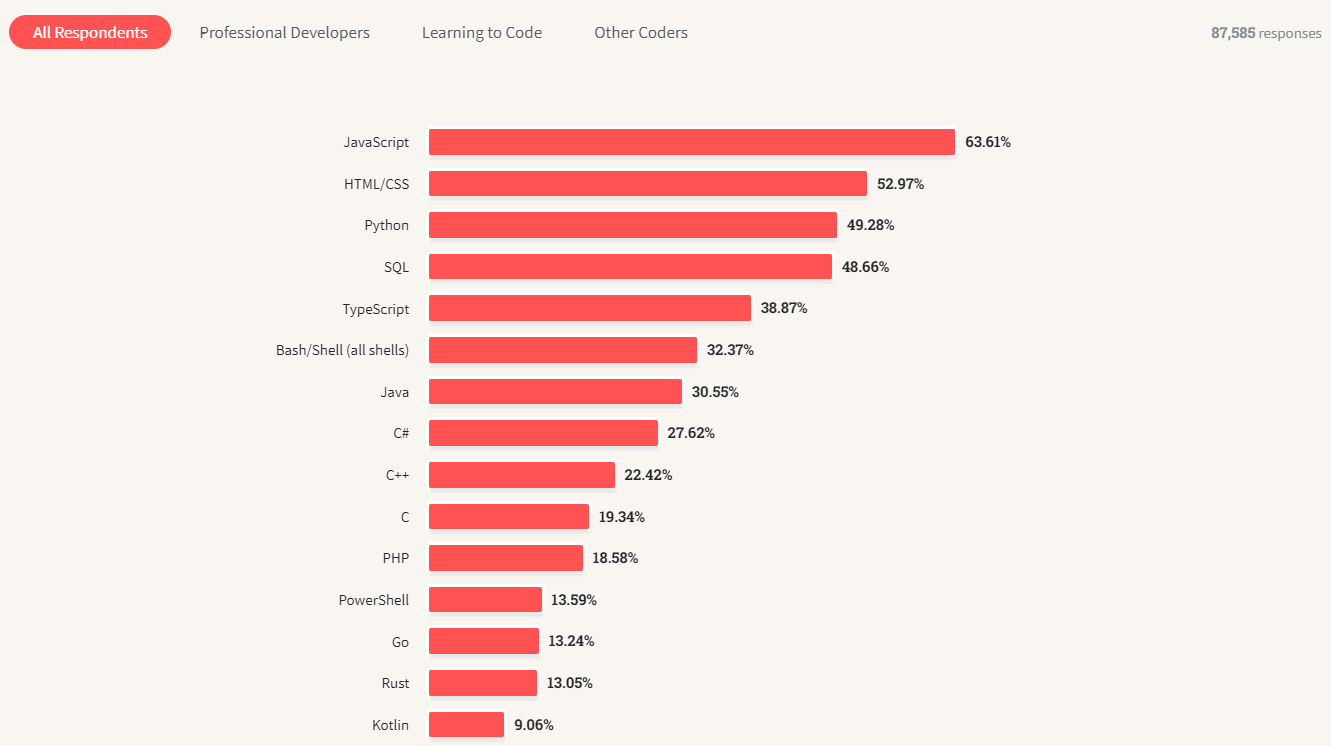
\includegraphics[width=160mm, keepaspectratio]{figures/go-stack-overflow.png}
    \caption{Most popular programming languages - 2023 Developer Survey by Stack Overflow}
\end{figure}

The language is designed to make programmers more productive in several fields, including  Web development, Cloud, Command Line (CLI) Applications, and DevOps, by offering modern features and a robust standard library. In most cases, you could write programs relying only on the standard library without using external dependencies. Nevertheless, the language ecosystem has a unique package management solution with an easy-to-use module system. You can download the packages from their package registry called pkg.go.dev\footnote{https://pkg.go.dev/} or even directly from a code repository like GitHub\footnote{https://github.com/}.

\subsection{Key features of Go}

The Go language has many features. I will introduce some of the most important ones in the following sub-sections: simplicity, readability, composition over inheritance, concurrency, tooling, and performance. 

\subsubsection{Simplicity}

The Go language is designed with simplicity in mind to address the complexity issue in software development. This feature was achieved by omitting common features in other languages and minimizing syntax. 

For example, Go only includes a \textbf{for} loop, leaving out constructs like \textbf{while} and \textbf{do-while}, and it lacks inheritance, a feature typical of object-oriented languages. Until a few versions ago, it was not even possible to write generic functions.

\subsubsection{Readability}

The language's minimal syntax makes it easy to read and understand, even for those who are not familiar with it firsthand. It can be a bit verbose compared to other languages, but this helps clarify the intent behind the code faster.

\subsubsection{Composition over inheritance \cite{gamma1994design}}

Composition over inheritance is a commonly applied design principle that promotes combining smaller, reusable components to achieve functionality rather than relying on hierarchical inheritance structures. The language does not have an inheritance feature at all. This approach reduces tight coupling and helps write more easily maintainable code.

\subsubsection{Tooling}

The language has an extensive set of tooling, including a compiler (go build), a package and dependency manager (go mod), a testing tool (go test), a code formatter (go fmt), and a language Server called (gopls\footnote{https://pkg.go.dev/golang.org/x/tools/gopls}). Most of them are deeply integrated into the ecosystem and come by default. Utilizing them, the developer could experience a fast, smooth, and efficient workflow experience.

\subsubsection{Concurrency}
Go features a simple yet robust concurrency model. It provides goroutines, lightweight threads managed by the Go runtime, and channels, facilitating safe and efficient communication between goroutines. It has an explicit syntax and is straightforward even for beginners, as the listing \ref{lst:goroutine} shows.

\begin{lstlisting}[caption=Calling a normal function as a goroutine,label=lst:goroutine, float]
package main

import (
	"fmt"
)

func normalFunction() {
	fmt.Println("I am a normal function")
}

func main() {
	// normal call
	normalFunction()

	// call as a goroutine
	go normalFunction()
}

\end{lstlisting}

\subsubsection{Performance}

Go is designed to be high-performance. This has been achieved by combining the speed of compiled programs with garbage-collector-based memory management. In addition, the concurrency model and the use of goroutines help to write fast and scalable applications.

\subsection{Advantages of using Go}

Go offers practical benefits that enhance software development and deployment. Its fast compile times speed up the development process, allowing more and faster iterations. Additionally, Go's ability to produce a single executable binary file simplifies the deployment process, even for different platforms.

Furthermore, Go's runtime includes a well-optimized garbage collector, which helps write applications with fewer memory leaks. Go's approach to treating errors as values is a simple and robust error-handling technique that forces developers to handle errors explicitly to reduce runtime failures.

\subsection{Disadvantages of using Go}

As with everything, Go has some disadvantages. The error-handling approach can be verbose and contain boilerplate code, as the developers must explicitly check and handle the errors.

I mentioned before that the language lacked generic functions and data types. It caused a lot of reimplementation of basic logic, e.g., the developers had to implement a linear search for every number type when deciding whether a slice contained it. The developer community still managed to convince the creators, and in 2022, version 1.18\footnote{https://go.dev/blog/why-generics} was released, which implemented this feature in some form, and since then, more and more features based on it have been released.

The language is not a multi-paradigm programming language; thus, you cannot write code in an object-oriented or functional style. This can be a deal breaker for those used to other modern languages like JavaScript, Python, Java, etc.

\section{Echo framework}

"Echo is an extensible, minimalist web framework for Go. It has a highly optimized router, offers a rich collection of middleware functions, and is one of the simplest solutions for writing a scalable web application"\cite{EchoFramework}.

\subsection{Key features}

Key features include automatic TLS, HTTP/2 support, a middleware system, and seamless integration with several templating engines. 

Echo's design centers on middleware, which enables developers to add authentication, logging, and other custom features with minimal configuration. The framework supports the creation of custom middleware, allowing developers to inject their logic into the request-handling pipeline. 

Besides the standard templating engine (html/template), Echo supports multiple third-party solutions such as htmgo\footnote{https://htmgo.dev/}, Jet\footnote{https://github.com/CloudyKit/jet}, and templ\footnote{https://github.com/a-h/templ} for generating dynamic HTML pages. Initially, this application used the standard library, but I later migrated the code to use the more type-safe solution templ, which I continue to use.

\subsection{Example}

Creating and starting an HTTP server with Echo requires three simple steps:
\begin{enumerate}
\item Instantiating an Echo instance
\item Registering middlewares and routes
\item Starting the server
\end{enumerate}

Listing~\ref{lst:echo-http-server} demonstrates these steps with code from the application:

\begin{lstlisting}[caption=Starting an Echo HTTP server,label=lst:echo-http-server, float]
package main

import (
    "github.com/labstack/echo/v4"
    "net/http"
)

func main() {
    // Instantiate the Echo
    e := echo.New()

    // Register a route handler that responds with an HTML page for requests coming from path /
    e.GET("/", func(c echo.Context) error {
        return render.TemplRender(c, http.StatusOK, pages.IndexPage())
    })

    // Start the server listening on the port 42069
    e.Start(":42069")
}

\end{lstlisting}

\section{SQLx and SQLc}

SQLx and SQLc are popular tools for working with SQL databases in Go. They take distinct approaches to handling database operations. The first one follows a more traditional approach by using type structures with tags and calling prepared statements. This methodology is known and commonly used in other languages and frameworks like Java Spring's Hibernate library\footnote{https://docs.spring.io/spring-framework/reference/data-access/orm/hibernate.html}. In contrast, the other generates the code directly from SQL schemas and queries containing prepared statements, ready-to-use data types, and type-safe functions for database access.

During the design phase, I used SQLx in the backend for database handling because its approach felt familiar based on my previous experiences. This familiarity was essential to me, given that most other tools used to build the platform were entirely new. However, later in the development, I learned about the SQLc library and tried it out. Half of the code still uses SQLx, but the other half is implemented with SQLc. As I became familiar with the Go ecosystem and its coding styles, I found SQLc more convenient, so I plan to migrate the entire codebase to SQLc.

\subsection{SQLx implementation approach}
As I mentioned, SQLx follows a traditional approach. The developers must create type structures with special tags called "struct tags" and write prepared statements with SQL queries within. They must also write Go code that calls the library and parses the results. This approach can be a better fit for developers who need more control and manual optimizations over the queries.

\subsection{SQLc implementation approach}
On the other hand, SQLc is a code generator with pros and cons. It is not just a library but a CLI program with various helping tools, and it supports other languages besides Go. 

The developers must write the SQL schema with special comments for the generator and the query. The compiler generates the proper data types, mappings, and type-safe functions that execute the desired query. To work like this, the compiler must have a simple yet easily extensible configuration file that describes the type conversions and the coding style in some sense. This approach is better for developers who prefer hiding complexity behind code generation or have to work on the same data model in different environments.

\section{templ}

The templ is a reasonably new, upcoming templating language library and CLI tool that helps create dynamic HTML fragments type-safely. It has a special JSX-like syntax, which became popular in the JavaScript ecosystem but uses a combination of Go and HTML. It is built on Go's standard templating solution, offering a better developer experience with a friendly syntax, convenient-to-use tools, and less error-prone, type-safe code generation.

\subsection{How does it work?}
Thus, it is a code-generation tool that allows for language extension with special syntax. In the world of templ, everything is a component written in a particular templ function in Go. These functions return templ components that render HTML text and can contain HTML code with some Go logic. The component functions have named and typed parameters like others, making them fully type-safe and compatible with code completion tools. Figure \ref{fig:templ-generation} shows the process of code generation from templ code.

\begin{figure}[!h]
    \centering
    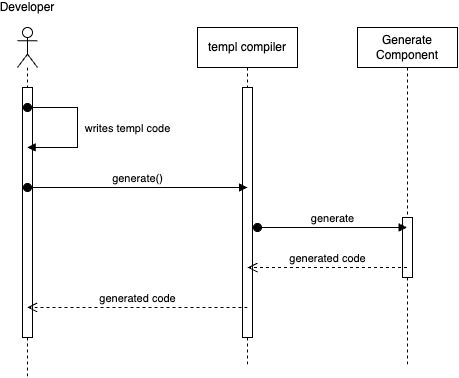
\includegraphics[width=0.8\textwidth, keepaspectratio]{figures/templ_sequence_generation.drawio.png}
    \caption{Code generation with templ compiler}
    \label{fig:templ-generation}
\end{figure}

Written code must follow strict coding rules and styles to generate the code called and used by the backend frameworks to render the page. The CLI contains a language server for code completion and syntax highlight, a code formatter, and a code generator tool. Figure \ref{fig:templ-rendering} shows the process of rendering a templ component.

\begin{figure}[!h]
    \centering
    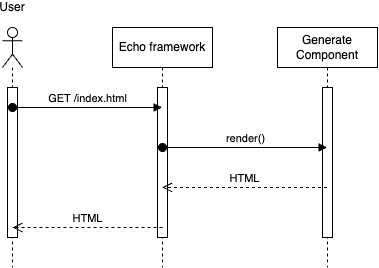
\includegraphics[width=0.8\textwidth, keepaspectratio]{figures/templ_sequence_render.drawio.png}
    \caption{Rendering templ component}
    \label{fig:templ-rendering}
\end{figure}

\section{HTMX}

HTMX is a tiny JavaScript library that allows developers to write server-rendered web applications primarily using HTML attributes. It enables HTML elements to handle advanced behaviors, eliminating or minimizing the need to write JavaScript code. It also complies with the REST constraint HATEOAS, as the returned HTML always contains the available actions for the requested resources.

One of the main goals is to create a SPA-like (single-page application) experience with the speed of server-rendered dynamic web pages. The difference between this and a traditional web application is the type of response. The communication is still based on HTTP, and the browser sends data in the known formats (URL, HTTP header, and HTTP body, even in JSON format), but the reactions are in HTML texts instead of JSON (or XML). The library is responsible for processing the HTML and updating the desired parts of the application based on the responses.

\subsection{Common HTMX attributes}

HTMX is like an extension of HTML, with 15 to 20 custom attributes that define how to process outgoing requests and incoming responses. The following ones are used the most.

Each HTTP method has attributes related to it: \textbf{hx-get}, \textbf{hx-post}, \textbf{hx-put}, \textbf{hx-patch}, \textbf{hx-delete}. Each one has one parameter: the URL where the request has to be sent when the actions happen. The listing \ref{lst:htmx-logout} shows performing a POST request to /logout on the default action of a button.

\begin{lstlisting}[caption=Preforming an \textbf{hx-post} request,label=lst:htmx-logout, float]
<button hx-post="/logout">Logout</button>
\end{lstlisting}

By default, on form submission, input value change, and button click, an HTMX request is performed when the method and URL are set. But there is a way to modify the default action trigger with \textbf{tx-trigger} attribute. It supports changing the event and allows the modifier to fine-grain the behavior, e.g., modifying an event, setting a delay, adding a throttle time, or filtering a key. The listing \ref{lst:htmx-trigger} shows performing a request on blur event with 300 ms of delay time.

\begin{lstlisting}[caption=Custom HTMX trigger,label=lst:htmx-trigger, float]
<input 
	id="data"
	name="data"
	type="text"
	hx-post="/update"
	hx-trigger="blur delay:300ms">
</input>
\end{lstlisting}

Some attributes define the process of the response. The two most common are \textbf{hx-target} and \textbf{hx-swap}; the first tells the library which element to swap, and the other tells how to do it. The target can be set by referring to the ID of the HTML element or using a CSS selector with special modifiers like \textbf{closest}, \textbf{next}, and \textbf{previous}. The other property tells how to do it, for example, changing the element's content, changing the whole element, and inserting before/after the target. The listing \ref{lst:htmx-target} shows a request, which response is replacing the element with id \textbf{\#page}.

\begin{lstlisting}[caption=Setting HTMX target,label=lst:htmx-target, float]
<a 
	hx-get="/home"
	hx-target="#page"
	hx-swap="outerHTML">Home
</a>
\end{lstlisting}

\subsection{Other attributes}
There are some cases when the website needs more complex logic, such as modifying multiple parts, sending additional data to the server, or doing client-side validation. HTMX offers solutions to all of them.

There are various methods to send data to the server, such as including it in the HTTP header or using the values from <input /> tags with \textbf{hx-include} or \textbf{hx-vals}.

If the application consists of several pages, navigation between them is necessary. This can be done with HTMX requests, in which the server sends not only the page but also the updated navigation bar. A request will cause the new page to appear and the navigation bar to be updated accordingly. This can be easily implemented with HTMX out-of-band requests\footnote{https://htmx.org/docs/#oob_swaps} and tags. The listing \ref{lst:htmx-oob} shows the request for a page and responses to the new page with the updated navigation bar.

\begin{lstlisting}[caption=Navigation with HTMX out-of-band request,label=lst:htmx-oob, float]
// The initial navigation bar
<nav
    id="navigation-bar"
    hx-target="#page"
    hx-swap="outerHTML"
>
    <a class="active" hx-get="/pages/1">Page one</a>
    <a hx-get="/pages/2">Page two</a> // the user clicks here
    <a hx-get="/pages/3">Page three</a>
</nav>

// the response containing the new page and an updated navigation bar
<div id="page">
    // Content of page two
</div>
<nav
    id="navigation-bar"
    hx-swap-oob="outerHTML:navigation-bar"
    hx-target="#page"
    hx-swap="outerHTML"
>
    <a hx-get="/pages/1">Page one</a>
    <a class="active" hx-get="/pages/2">Page two</a> // .active class is applied
    <a hx-get="/pages/3">Page three</a>
</nav>

\end{lstlisting}

Doing client-side validation, getting a prompt, or getting a confirmation from the user before sending a request, is easy; it just needs setting \textbf{hx-validate} and \textbf{hx-prompt} or \textbf{hx-confirm} attributes, respectively.

\section{Other technologies and tools}

TODO decide whether this section is even needed:

TODO normal tools:
node, docker, tailwindcss, ollama

TODO ai tools:
v0, copilot, claude/gippity
